\documentclass{article}
\usepackage[utf8]{inputenc}
\usepackage{amsmath}
\usepackage{indentfirst}
\usepackage{graphicx,caption}
\usepackage[a4paper, margin=1in]{geometry}
\linespread{1.15}
\usepackage{empheq}
\usepackage[most]{tcolorbox}
\usepackage[margin=3cm]{caption}
\usepackage{siunitx}
\usepackage{array}
\usepackage{braket}
\usepackage{mathtools}

\usepackage{xcolor,sectsty}
\definecolor{astral}{RGB}{46,116,181}
\subsectionfont{\color{astral}}
\sectionfont{\color{astral}}

\title{
\includegraphics[width=0.1\textwidth]{ufallogo.png} \\
\Huge{\color{astral}\textbf{Informação Quântica}}}
\author{Paulo Brandão}
\date{Maio de 2017}

\newtcbox{\mymath}[1][]{%
    nobeforeafter, math upper, tcbox raise base,
    enhanced, colframe=blue!30!black,
    colback=blue!30, boxrule=1pt,
    #1}
\newcommand*{\bfrac}[2]{\genfrac{\lbrace}{\rbrace}{0pt}{}{#1}{#2}}
\begin{document}

\maketitle

\section{Introdução}

Uma teoria quantitativa da informação surgiu na ciência em 1948 com o trabalho de Claude Shannon intitulado \textit{Uma Teoria Matemática da Comunicação}. Neste trabalho seminal, Shannon conseguiu obter uma expressão para o conteúdo informativo de uma mensagem, chamada de \textit{Entropia de Shannon}. Além disso, demonstrou matematicamente dois importantes teoremas que relacionam a transmissão dessa informação entre duas partes através de canais de comunicação com ou sem ruído. A grande ideia por trás do trabalho de Shannon foi a profunda associação do conteúdo informativo de uma mensagem com o grau de incerteza, isto é, com a probabilidade, envolvida no processo de obtenção dos caracteres da mensagem. O fato de que a probabilidade depende do conhecimento do indivíduo já era conhecido desde a época de Bayes e pode ser demonstrado por um exemplo muito simples: Se Bob coloca um prêmio dentro de uma de três caixas disponíveis e pede para que Alice escolha uma das caixas, ganhando o prêmio se acertar a caixa na qual o prêmio está, a probabilidade de acerto para Bob é 1 (ele sabe em qual caixa encontrar o prêmio) mas para Alice é 1/3. Assim, probabilidade é um conceito relativo que depende da ignorância da pessoa com relação ao determinado evento.

A mecânica quântica, desenvolvida antes das ideias de Shannon aparecerem na literatura, envolve justamente o conceito de probabilidade de uma maneira fundamental. Toda a teoria quântica é probabilística. Dessa forma é natural esperar que uma teoria quântica da informação fosse formulada em algum momento. Da mesma forma em que é possível quantificar o conteúdo informativo de uma mensagem clássica, podemos quantificar o conteúdo informativo de um estado quântico. A mecânica quântica pode ser utilizada para processar e transmitir informação. A grande diferença entre o processamento e a transmissão de informação quântica quando comparado com os mesmos processos num regime clássico é que no mundo microscópico as leis físicas são diferentes. Classicamente, podemos representar qualquer mensagem através da base binária $\{ 0,1 \}$ cujos elementos são chamados de bits. Uma canal de comunicação clássico transmite informação através da emissão de sinais analógicos ou digitais baseados na base binária. É dessa forma que um computador trabalha. Na eletrônica digital, por exemplo, o elemento 0 representa uma voltagem nula enquanto que o elemento 1 representa uma voltagem de aproximadamente 5 volts numa sequência de pulsos eletrônicos que são transmitidos e recebidos pelos transistores. Como qualquer número pode ser representado através da base binária, é possível transmitir qualquer tipo de informação clássica utilizando 0's e 1's.

Um canal de comunicação quântico, por outro lado, tem muito mais liberdade na escolha de sua base binária, cujos elementos são chamados neste caso de \textit{qubits}: $\{ \ket{0},\ket{1} \}$. Isso se deve ao fato de que os sistemas físicos, quando observados na escala microscópica, exibem o fenômeno de \textit{superposição quântica}. Com apenas dois qubits podemos representar infinitos estados do tipo 
\begin{equation}
    \ket{\psi} = c_1 \ket{0} + c_2 \ket{1},
\end{equation}
um para cada valor escolhido de $c_i$ de tal forma que $|c_1|^2 + |c_2|^2 = 1$. No entanto, uma medida do estado $\ket{\psi}$ pode nos dar apenas os valores 0 ou 1 com as respectivas probabilidades $|c_1|^2$ e $|c_2|^2$. Além da possibilidade de superposição de estados quânticos, a natureza também permite o \textit{entrelaçamento quântico}, onde um sistema formado por duas ou mais partes possui correlações entre suas entidades primárias mesmo que estejam localizadas em diferentes cidades! Essas duas propriedades, superposição e entrelaçamento, formam o coração da teoria quântica da informação e são as responsáveis pelas grandes diferenças encontradas entre as teorias clássica e quântica. 

Nesta aula irei apresentar os aspectos básicos da transmissão da informação através de circuitos quânticos. Ou seja, estarei interessado principalmente na atuação de portas lógicas quânticas e como elas podem ser implementadas para transmitir informação. Essa subárea da extensa linha de pesquisa \textit{informação quântica} é extremamente importante e é geralmente o primeiro contato que o estudante tem com essa área de estudo. Um dos grandes objetivos da transmissão de informação quântica é, claro, verificar a possibilidade de construção de um computador quântico. Tentarei expor os princípios por trás desta implementação. 


\section{Eletrônica digital}

Computadores operam através de sequências binárias formadas por elementos chamados de \textit{bits} consistindo em 0's e 1's. Um elemento eletrônico de uma placa pode ler a lista de bits e processar o resultado através de tarefas eletrônicas. Claro que é necessário um processo físico para gerar essa lista de caracteres binários. Na eletrônica digital, uma série de pulsos, regularmente espaçados, é utilizada para criar a lista binária. Assim, um pulso com amplitude de voltagem 0 Volts representa o bit $0$ e um pulso com amplitude de voltagem geralmente igual a $5$ Volts representa o bit $1$:
\begin{center}
    \begin{verbatim}
     Pulso no tempo:   _-__--_---_-__-_-     =>     01001101110100101
    \end{verbatim}
\end{center}
Como qualquer caractere pode ser representado pela base binária, esse procedimento pode ser utilizado para transmitir todo tipo de informação clássica. É claro que para criar um tipo específico de lista binária para ser transmitida, é necessária a atuação do sistema físico no processo. Essa atuação é descrita pelas \textbf{portas lógicas}. Vamos supor, por exemplo, que um elemento do circuito tem a função de acender um led quando o mesmo receber um bit $0$. Se estivermos apenas de posse da sequência binária
\begin{center}
    \begin{verbatim}
                     ...-------------...     =>     ...111111111111...
    \end{verbatim}
\end{center}
nunca conseguiremos acender o led desejado (os três pontinhos indicam que a sequência se repete indefinidamente). É necessária a atuação de um outro elemento físico para mudar o estado de, pelo menos um bit, de 1 para 0. A porta lógica é um conceito teórico que representa o agente físico capaz de fazer essa mudança em um ou mais bits numa sequência. É fácil concluir que só existem dois tipos de ações que uma porta lógica clássica pode fazer ao receber um bit de entrada:
\begin{itemize}
    \item Inverter o valor do bit.
    \item Não fazer nada com o bit.
\end{itemize}
A porta lógica \textbf{NOT} representa o sistema físico que inverte o bit de entrada, isto é, sua operação é descrita pela tabela verdade:
\begin{center}
\begin{tabular} { |c|c|  }
 \hline
 \multicolumn{2}{|c|}{Porta \textbf{NOT}} \\
 \hline
 Entrada & Saída\\
 \hline
 0   & 1\\
 1   & 0\\
 \hline
\end{tabular}
\end{center}
Representamos essa ação através do diagrama

\begin{center}
    \begin{verbatim}
                                1-------|NOT|-------0
                                0-------|NOT|-------1
    \end{verbatim}
\end{center}
que deve ser lido da esquerda para a direita. Um elemento do circuito pode atuar ainda em dois bits ao mesmo tempo. Isto é, dependendo dos valores dos bits $A$ e $B$, tomados em conjunto, uma certa operação será feita. A porta lógica \textbf{OR} possui a seguinte tabela verdade:

\begin{center}
\begin{tabular} { |c|c|c|  }
 \hline
 \multicolumn{3}{|c|}{Porta \textbf{OR}} \\
 \hline
 Entrada A & Entrada B & Saída\\
 \hline
 0 & 0 & 0\\
 0 & 1 & 1\\
 1 & 0 & 1\\
 1 & 1 & 1 \\
 \hline
\end{tabular}
\end{center}
Isto é, se e somente se um dos bits de entrada for 1, o resultado é um bit 1. Caso contrário, a saída é um bit 0. Já a porta lógica \textbf{AND} possui a seguinte tabela verdade

\begin{center}
\begin{tabular} { |c|c|c|  }
 \hline
 \multicolumn{3}{|c|}{Porta \textbf{AND}} \\
 \hline
 Entrada A & Entrada B & Saída\\
 \hline
 0 & 0 & 0\\
 0 & 1 & 0\\
 1 & 0 & 0\\
 1 & 1 & 1 \\
 \hline
\end{tabular}
\end{center}
 
A imaginação vai longe nas possibilidades de criação das portas lógicas. Porém, existe uma porta muito importante que deve ser mencionada: A porta lógica \textbf{NOT-AND} ou \textbf{NAND}:

\begin{center}
\begin{tabular} { |c|c|c|  }
 \hline
 \multicolumn{3}{|c|}{Porta \textbf{NAND}} \\
 \hline
 Entrada A & Entrada B & Saída\\
 \hline
 0 & 0 & 1\\
 0 & 1 & 1\\
 1 & 0 & 1\\
 1 & 1 & 0 \\
 \hline
\end{tabular}
\end{center}
Essa porta tem a interessante propriedade de ser \textit{universal}. Todas as operações de computação podem ser realizadas utilizando apenas portas \textbf{NAND}. De fato, você pode construir um computador completo utilizando apenas portas \textbf{NAND}, ou uma combinação das portas \textbf{NOT} e \textbf{AND}. Um circuito clássico é criado através da junção de várias portas lógicas para desempenhar uma determinada tarefa. Esse é o ponto de partida da álgebra Booleana, desenvolvida por George Boole, e que forma os fundamentos da computação clássica numa linguagem matemática. Não devemos esquecer, portanto, que todas as operações binárias executadas por um computador clássico envolvem voltagens transmitidas por uma corrente elétrica que são manipuladas por dispositivos formados por transistores (são os transistores que representam fisicamente as propriedades das portas descritas aqui). Nosso próximo objetivo é visualizar o computador numa escala cada vez menor de modo que o mesmo seja regido pelas leis da mecânica quântica. Para isso, precisamos inicialmente generalizar o conceito de bit clássico para o bit quântico e verificar de que maneira podemos manipular o bit quântico através de portas lógicas.





\section{Portas lógicas quânticas}

No processamento de informação \textbf{quântica}, os valores lógicos 0 e 1 são substituídos pelos estados ortogonais $\ket{0}$ e $\ket{1}$ chamados \textit{qubits}. No entanto, diferente do caso clássico onde apenas 0 ou 1 podem ser transmitidos, para sistemas microscópicos é possível descrever o estado geral $\ket{\psi}$ de um qubit através da superposição dos estados $\ket{0}$ e $\ket{1}$:
\begin{equation}
    \ket{\psi} = a\ket{0} + b\ket{1}
    \label{super}
\end{equation}
com $|a|^2 + |b|^2 = 1$. Ao fazer uma medida do estado $\ket{\psi}$, entretanto, apenas os valores $\ket{0}$ ou $\ket{1}$ são obtidos com as respectivas probabilidades $|a|^2$ e $|b|^2$. Entre o preparo e a medida da informação, ela reside no estado quântico do sistema que evolui de acordo com o Hamiltoniano. A mecânica quântica permite a ação de qualquer transformação unitária no qubit e podemos portanto identificar a ação de \textbf{portas quânticas} com operadores unitários que desempenham certas tarefas, como ilustra o diagrama abaixo

\begin{center}
    \begin{verbatim}
                                |k> -------|U|------- U|k> 
    \end{verbatim}
\end{center}
O operador unitário $\hat{U}$ faz o papel de uma porta quântica que irá manipular qubits de entrada $\ket{k}$ transformando-os em qubits $\hat{U}\ket{k}$ de saída. É útil utilizar a representação matricial para os qubits $\ket{0}$ e $\ket{1}$ que formam a \textbf{base computacional padrão}:
\begin{equation}
\ket{0} = 
    \begin{bmatrix}
    1\\
    0
    \end{bmatrix}, 
    \hspace{0.5cm}
    \ket{1} = 
    \begin{bmatrix}
    0\\
    1
    \end{bmatrix}
\end{equation}
e o estado geral, dado pela superposição \eqref{super}, pode ser escrito na forma matricial
\begin{equation}
\ket{\psi} = a \begin{bmatrix}
    1\\
    0
    \end{bmatrix} + b \begin{bmatrix}
    0\\
    1
    \end{bmatrix}
    =
    \begin{bmatrix}
    a\\
    b
    \end{bmatrix}.
\end{equation}
De posse do estado arbitrário de um qubit de entrada, podemos definir as \textbf{portas quânticas} mais utilizadas e verificar a sua ação na base computacional padrão.
 
\subsection{Porta quântica \textbf{NOT}}

A porta quântica \textbf{NOT} é definida como a ação física que transforma o bit $\ket{0}$ em $\ket{1}$ e vice-versa, análogo ao caso clássico. Seu diagrama é representado na forma
\begin{center}
    \begin{verbatim}
                                |1> -------|NOT|------- |0> 
                                |0> -------|NOT|------- |1>                                 
    \end{verbatim}
\end{center}
e o operador unitário responsável por essa ação pode ser escrito na forma matricial 
\begin{equation}
    \hat{X} = \begin{bmatrix}
    0 & 1\\
    1 & 0
    \end{bmatrix},
\end{equation}
onde vê-se facilmente que a operação é unitária $\hat{U}^\dagger \hat{U} = \hat{I}$. Se um estado qubit $\ket{\psi}$ passar por uma porta quântica \textbf{NOT}, a ação resultante é facilmente calculada:
\begin{equation}
    \ket{\psi} = a\ket{0} + b\ket{1} \longrightarrow \hat{X}\ket{\psi} = 
    \begin{bmatrix}
    0 & 1\\
    1 & 0
    \end{bmatrix}
    \begin{bmatrix}
    a\\
    b
    \end{bmatrix} = 
    \begin{bmatrix}
    b\\
    a
    \end{bmatrix} = a\ket{1} + b\ket{0}.
\end{equation}
Se medirmos o estado do qubit $\ket{\psi}$ após o mesmo passar por uma porta \textbf{NOT}, obtemos o qubit $\ket{1}$ com probabilidade $|a|^2$ e o qubit $\ket{0}$ com probabilidade $|b|^2$, que são valores \textit{diferentes} para o estado do qubit inicial! A porta quântica \textbf{NOT} troca, portanto, os valores das medidas das probabilidades para os dois estados da base computacional.

O estudante mais atento pode ter percebido que a matriz unitária representada pelo operador $\hat{X}$ nada mais é que uma das matrizes de Pauli $\sigma_x$. Todas as 3 matrizes de Pauli são unitárias e podem, portanto, representar operações unitárias em qubits de entrada. A outra matriz de Pauli, geralmente nomeada de $\sigma_y$, pode representar a ação unitária
\begin{equation}
    \hat{Y} = \begin{bmatrix}
    0 & -i\\
    i & 0
    \end{bmatrix},
\end{equation}
cujo efeito num qubit genérico de entrada $\ket{\psi}$ é
\begin{equation}
    \hat{Y}\ket{\psi} = a\hat{Y}\ket{0} + b \hat{Y}\ket{1} = -ib\ket{0} + ia\ket{1}.
\end{equation}
A ação do operador unitário restante, representado pela matriz de Pauli $\sigma_z$, pode ser facilmente verificada pelo estudante através da resolução da lista de exercício.

\subsection{Porta quântica Hadamard}

A porta quântica Hadamard é uma das mais utilizadas em teoria computacional quântica e é definida pela seguinte matriz unitária
\begin{equation}
    \hat{H} = \frac{1}{\sqrt{2}}\begin{bmatrix}
    1 & 1\\
    1 & -1
    \end{bmatrix}.
\end{equation}
A ação da porta Hadamard na base computacional $\{ \ket{0},\ket{1} \}$ é facilmente calculada:
\begin{equation}
    \hat{H}\ket{0} = 
    \frac{1}{\sqrt{2}}\begin{bmatrix}
    1 & 1\\
    1 & -1
    \end{bmatrix}
    \begin{bmatrix}
    1\\
    0
    \end{bmatrix} = 
    \frac{1}{\sqrt{2}}\begin{bmatrix}
    1\\
    1
    \end{bmatrix} = \frac{1}{\sqrt{2}}(\ket{0} + \ket{1})
\end{equation}
e
\begin{equation}
    \hat{H}\ket{1} = 
    \frac{1}{\sqrt{2}}\begin{bmatrix}
    1 & 1\\
    1 & -1
    \end{bmatrix}
    \begin{bmatrix}
    0\\
    1
    \end{bmatrix} = 
    \frac{1}{\sqrt{2}}\begin{bmatrix}
    1\\
    -1
    \end{bmatrix} = \frac{1}{\sqrt{2}}(\ket{0} - \ket{1}).
\end{equation}
Sua ação num qubit arbitrário $\ket{\psi}$ é dada por
\begin{equation}
    \hat{H}\ket{\psi} = a\hat{H}\ket{0} + b\hat{H}\ket{1} = \frac{a}{\sqrt{2}}(\ket{0} + \ket{1}) + \frac{b}{\sqrt{2}}(\ket{0} - \ket{1}) = \frac{a+b}{\sqrt{2}}\ket{0} + \frac{a-b}{\sqrt{2}}\ket{1}.
\end{equation}
Dessa forma, se medirmos o estado do qubit $\ket{\psi}$ após o mesmo passar por uma porta quântica do tipo Hadamard, obtemos como resultado o qubit $\ket{0}$ com probabilidade $|a+b|^2/2$ e o qubit $\ket{1}$ com probabilidade $|a-b|^2/2$. Note que mesmo se os qubits de entrada forem apenas os estados $\ket{0}$ ou $\ket{1}$, a ação da porta Hadamard é colocá-los numa superposição quântica. Se o qubit $\ket{0}$ (ou $\ket{1}$) não sofresse a ação da porta Hadamard, sua medida iria retornar o valor 0 (ou 1) com 100\% de certeza. Após passar pela porta, no entanto, a probabilidade de se obter 1 ou 0 cai para 50\%. 

\subsection{Portas controladas}

As portas quânticas descritas anteriormente atuam somente em um qubit de entrada fornecendo um único qubit de saída. Esse tipo de porta é chamado de porta de um qubit. Quando uma porta quântica permite a entrada de \textit{dois} qubits, as coisas ficam muito mais interessantes. Antes de introduzirmos algumas portas quânticas de dois qubits, é útil verificar como podemos descrever dois qubits algebricamente. Assumimos que um dos qubits que irá entrar na porta quântica pertence ao espaço de Hilbert (de dimensão 2) $\mathcal{H}_1$ e o outro qubit pertence ao espaço de Hilbert (também de dimensão 2) $\mathcal{H}_2$. O estado do \textit{sistema} formado pelos dois qubits é descrito por vetores pertencentes ao espaço de Hilbert formado pelo produto tensorial $\mathcal{H} = \mathcal{H}_1 \otimes \mathcal{H}_2$. O estado $\ket{\psi}$ de dois qubits é descrito como
\begin{equation}
    \ket{\Psi} = \ket{\psi}_1 \otimes \ket{\psi}_2 = \ket{\psi_1 \psi_2}
\end{equation}
onde a notação utilizada indica que o primeiro termo dentro do ket, $\ket{(\text{esse termo})(\cdot)}$, pertence ao espaço $\mathcal{H}_1$ e o segundo termo, $\ket{(\cdot)(\text{esse termo})}$, pertence ao espaço $\mathcal{H}_2$. Uma base para o espaço $\mathcal{H}$ pode ser formada a partir da base qubit $\ket{1}$ e $\ket{0}$ de cada espaço:
\begin{equation}
    \ket{11} = \ket{1}_1 \otimes \ket{1}_2 = 
    \begin{bmatrix}
    0\\
    1
    \end{bmatrix}
    \otimes\begin{bmatrix}
    0\\
    1
    \end{bmatrix} = 
    \begin{bmatrix}
    0\begin{bmatrix}
    0\\
    1
    \end{bmatrix}\\
    1\begin{bmatrix}
    0\\
    1
    \end{bmatrix}
    \end{bmatrix} = \begin{bmatrix}
    0 \cdot 0\\
    0 \cdot 1\\
    1 \cdot 0\\
    1 \cdot 1\\
    \end{bmatrix} = \begin{bmatrix}
    0\\
    0\\
    0\\
    1\\
    \end{bmatrix}
\end{equation}

\begin{equation}
    \ket{10} = \ket{1}_1 \otimes \ket{0}_2 = 
    \begin{bmatrix}
    0\\
    1
    \end{bmatrix}
    \otimes\begin{bmatrix}
    1\\
    0
    \end{bmatrix} = 
    \begin{bmatrix}
    0\begin{bmatrix}
    1\\
    0
    \end{bmatrix}\\
    1\begin{bmatrix}
    1\\
    0
    \end{bmatrix}
    \end{bmatrix} = \begin{bmatrix}
    0 \cdot 1\\
    0 \cdot 0\\
    1 \cdot 1\\
    1 \cdot 0\\
    \end{bmatrix} = \begin{bmatrix}
    0\\
    0\\
    1\\
    0\\
    \end{bmatrix}
\end{equation}

\begin{equation}
    \ket{01} = \ket{0}_1 \otimes \ket{1}_2 = 
    \begin{bmatrix}
    1\\
    0
    \end{bmatrix}
    \otimes\begin{bmatrix}
    0\\
    1
    \end{bmatrix} = 
    \begin{bmatrix}
    1\begin{bmatrix}
    0\\
    1
    \end{bmatrix}\\
    0\begin{bmatrix}
    0\\
    1
    \end{bmatrix}
    \end{bmatrix} = \begin{bmatrix}
    1 \cdot 0\\
    1 \cdot 1\\
    0 \cdot 0\\
    0 \cdot 1\\
    \end{bmatrix} = \begin{bmatrix}
    0\\
    1\\
    0\\
    0\\
    \end{bmatrix}
\end{equation}

\begin{equation}
    \ket{00} = \ket{0}_1 \otimes \ket{0}_2 = 
    \begin{bmatrix}
    1\\
    0
    \end{bmatrix}
    \otimes\begin{bmatrix}
    1\\
    0
    \end{bmatrix} = 
    \begin{bmatrix}
    1\begin{bmatrix}
    1\\
    0
    \end{bmatrix}\\
    0\begin{bmatrix}
    1\\
    0
    \end{bmatrix}
    \end{bmatrix} = \begin{bmatrix}
    1 \cdot 1\\
    1 \cdot 0\\
    0 \cdot 1\\
    0 \cdot 0\\
    \end{bmatrix} = \begin{bmatrix}
    1\\
    0\\
    0\\
    0\\
    \end{bmatrix},
\end{equation}
assim, a base computacional do sistema descrito por um estado $\ket{\Psi}$ pertencente ao espaço de Hilbert $\mathcal{H}$ é dada por
\begin{equation}
    \{ \ket{00},\ket{01},\ket{10},\ket{11} \}
\end{equation}
cujas representações matriciais estão descritas acima. Fica claro então que um portâo quântico $\hat{U}$ atuando sob um sistema de dois qubits será descrito por uma matriz $4\times 4$ já que a dimensão do espaço $\mathcal{H}$ é 4. O estado geral de um sistema formado por dois qubits pode ser expandido em termos dos estados da base na forma
\begin{equation}
    \ket{\psi} = a\ket{00} + b\ket{01} + c\ket{10} + d\ket{11} = \begin{bmatrix}
    a\\
    b\\
    c\\
    d\\
    \end{bmatrix}.
    \label{estadogeral}
\end{equation}

As portas quânticas mais úteis que recebem dois qubits e executam uma determinada função são as portas controladas. Suponha que uma porta quântica aceite dois qubits de entrada e defina um dos qubits como sendo o \textit{qubit controle} e o outro como sendo o \textit{qubit alvo}. Considere inicialmente o caso especial onde o qubit de entrada é $\ket{\psi} = \ket{00}$, ou seja, a porta recebe dois qubits, um no estado $\ket{0}_1$ e o outro no estado $\ket{0}_2$. Vamos definir o qubit do espaço $\mathcal{H}_1$ como o qubit controle e o outro qubit do espaço $\mathcal{H}_2$ como o qubit alvo. A ação da porta \textbf{CNOT} (\textbf{C}ontrolled-\textbf{NOT}) é a seguinte:
\begin{itemize}
    \item Se o qubit controle for 0, nada acontece.
    \item Se o qubit controle for 1, inverta o estado do qubit alvo.
\end{itemize}
Como assumimos que o estado de entrada é $\ket{\psi} = \ket{00}$ onde o qubit controle é 0, nada irá acontecer e o qubit de saída será $\ket{00}$. O mesmo comportamento ocorre se o qubit de entrada for o estado $\ket{01}$: como o qubit controle é 0, nada acontece e o estado na saída da porta quântica é o mesmo estado que entrou. Por outro lado, se o estado de entrada for $\ket{10}$, o qubit de controle é 1 e a porta quântica inverte o estado do qubit alvo resultando no estado de saída $\ket{11}$. O mesmo comportamento acontece quando o estado de entrada for $\ket{11}$, resultando no estado de saída $\ket{10}$. É fácil verificar que a ação da porta quântica \textbf{CNOT} no estado geral \eqref{estadogeral} tem o efeito de trocar $c$ por $d$ (verifique!). É útil representar a ação da porta \textbf{CNOT} através do diagrama 
\begin{figure}[ht]
\centering
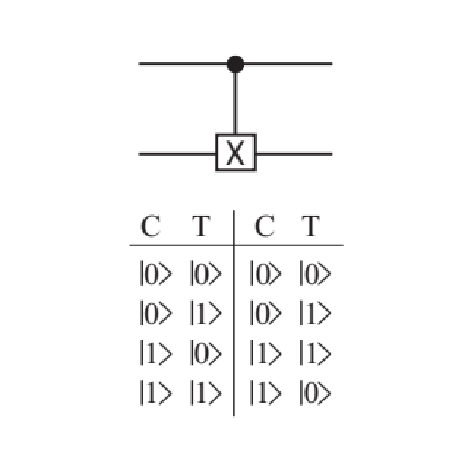
\includegraphics[width=5cm]{fig1novo.pdf}
\captionsetup{labelsep=none}
\caption{. Representação esquemática da porta quântica \textbf{CNOT}. As duas linhas horizontais representam qubits de cada espaço de Hilbert. A linha superior indica o qubit controle pertencente ao espaço $\mathcal{H}_1$ enquanto que a linha inferior indica o qubit alvo pertencente ao espaço $\mathcal{H}_2$. Para indicar o qubit controle utiliza-se um ponto preenchido e para indicar o qubit alvo utiliza-se um círculo em forma de cruz. A tabela verdade para o portão está mostrada na parte inferior da figura. Note que a figura deve ser ``lida'' da esquerda para a direita.}
\end{figure}
A representação matricial do operador unitário $\hat{U}_\text{CN}$ é dada pela seguinte matriz $4\times 4$:
\begin{equation}
    \hat{U}_{\text{CN}} = \begin{bmatrix}
    1 & 0 & 0 & 1\\
    0 & 1 & 0 & 0\\
    0 & 0 & 0 & 1\\
    0 & 0 & 1 & 0\\
    \end{bmatrix},
\end{equation}
que pode ser facilmente verificada através da atuação nas matrizes da base computacional descritas no início desta seção.

É claro que existem vários tipos de portas controladas. O exemplo anterior utilizou a porta \textbf{NOT} para atuar no qubit alvo. Mas podemos utilizar a imaginação e permitir a atuação da porta quântica no qubit alvo com qualquer tipo de porta de um qubit. Por exemplo, podemos criar a porta quântica que atua da seguinte maneira:
\begin{itemize}
    \item Se o qubit controle for 0, nada acontece.
    \item Se o qubit controle for 1, o qubit alvo passa por uma porta Hadamard.
\end{itemize}
Se o estado de entrada for $\ket{00}$ nada acontece pois o qubit controle é 0. O mesmo ocorre quando o estado de entrada é $\ket{01}$. Por outro lado, se o estado de entrada for $\ket{10}$, o qubit alvo, $\ket{0}_2$, sofre a transformação unitária
\begin{equation}
    \hat{H}\ket{0}_2 = \frac{1}{\sqrt{2}}(\ket{0}_2 + \ket{1}_2)
\end{equation}
resultando no qubit de saída
\begin{equation}
    \ket{\psi}_\text{out} = \ket{1}\otimes \hat{H}\ket{0}_2 = \frac{1}{\sqrt{2}}(\ket{10} + \ket{11}).
\end{equation}
Se uma medida for efetuada no estado de saída, podemos encontrar o qubit do espaço $\mathcal{H}_1$ e o qubit do espaço $\mathcal{H}_2$ nos estados 1 e 0, respectivamente, com probabilidade de 50\% ou o qubit do espaço $\mathcal{H}_1$ e o qubit do espaço $\mathcal{H}_2$ nos estados 1 e 1 com probabilidade de 50\%. A representação esquemática dessa porta, que podemos chamar de \textbf{CH} (\textbf{C}ontrolled-\textbf{H}adamard), é a mesma da Figura 1 com a troca do $X$, que representa o \textbf{NOT}, pelo $H$ que representa Hadamard.





\section{Circuitos quânticos}

Assim como a junção das portas lógicas clássicas dão origem aos circuitos digitais, a junção de portas quânticas geram os circuitos quânticos. A primeira conexão do estudante com circuitos se dá por meio do eletromagnetismo, onde o estudante aprende como funciona um resistor, depois um capacitor e por fim um indutor. Colocando todos esses elementos para trabalhar em conjunto, é possível desenvolver tarefas específicas e extremamente úteis com aplicações em eletrônica. Da mesma forma, a junção de portas quânticas nos permite desenvolver circuitos quânticos que podem ser muito úteis de um ponto de vista prático. A construção de um computador quântico só será possível através do estudo e desenvolvimento de circuitos quânticos viáveis.

Vamos dar apenas um exemplo de um circuito quântico cuja finalidade é gerar um \textit{estado de Bell} com os conceitos e as portas discutidas nas secões anteriores. Suponha que nosso objetivo seja construir, a partir de um estado de entrada $\ket{\psi}_i$, um estado de saída que seja um estado de Bell do tipo
\begin{equation}
    \ket{\psi}_f = \frac{1}{\sqrt{2}}(\ket{01} + \ket{10}).
\end{equation}
Se medirmos o estado do qubit no espaço $\mathcal{H}_1$ e encontrarmos que ele vale 1, então sabemos que o estado do qubit no espaço $\mathcal{H}_2$ vale \textit{instantâneamente} 0 e vice-versa. Essa propriedade não-local da mecânica quântica está ligada com o fato de que o estado de Bell acima não pode ser fatorado na forma $\ket{\cdot}_1 \otimes \ket{\cdot}_2$, isto é, ele representa um estado \textit{emaranhado}. O princípio da superposição (que já vemos utilizando desde o início da análise) e as propriedades de emaranhamento dos estados, são os dois conceitos que mudam completamente o comportamento dos sistemas de informação quânticos comparados com a informação clássica.

Suponha que o estado de entrada seja $\ket{\psi}_i = \ket{01}$, isto é, o estado do qubit controle é $\ket{0}_1$ e o estado do qubit alvo é $\ket{1}_2$, onde os índices indicam os espaços de Hilbert. Vamos introduzir o estado inicial do sistema no seguinte circuito quântico:
\begin{figure}[ht]
\centering
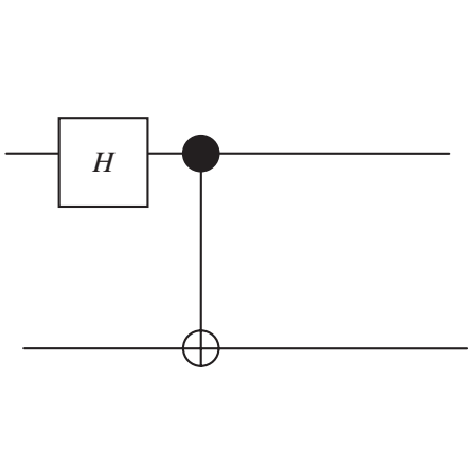
\includegraphics[width=5cm]{fig2novo.pdf}
\captionsetup{labelsep=none}
\caption{. Circuito quântico utilizado para gerar os estados de Bell. O qubit controle passa por uma porta Hadamard antes de ser submetido, junto com o qubit alvo, através de uma porta \textbf{CNOT}.}
\end{figure}
Observe que apenas o qubit controle (que pertence ao espaço de Hilbert $\mathcal{H}_1$) passa pela porta Hadamard. Se o estado inicial for $\ket{\psi}_i = \ket{01} = \ket{0}_1\otimes\ket{1}_2$, o estado do sistema após o qubit controle passar pela porta Hadamard é dado por
\begin{equation}
    \ket{\psi}_m = \left[ \frac{1}{\sqrt{2}}(\ket{0}_1 + \ket{1}_1) \right] \otimes \ket{1}_2 = \frac{1}{\sqrt{2}}(\ket{01} + \ket{11}).
\end{equation}
Dessa forma, a porta \textbf{CNOT} receberá o estado $\ket{\psi}_m$ como entrada e produzirá o estado de saída 
\begin{equation}
    \ket{\psi}_f = \frac{1}{\sqrt{2}}(\ket{01} + \ket{10}) 
\end{equation}
que representa um dos estados de Bell. O circuito representado na Figura 2 pode ser utilizado portanto para produzir estados emaranhados a partir de estados separáveis (neste exemplo o estado inicial foi $\ket{\psi}_i =\ket{01}$).

Pode parecer que seja necessário criar infinitos tipos de portas para executar tarefas mais complicadas. Isso, no entanto, não é verdade. É possível demonstrar que todo circuito com 3-qubits de entrada, por exemplo, pode ser representado pela ação de várias portas de 2-qubit. Da mesma forma que existem portas universais no sistema clássico, também existem portas universais no processamento de informação quântica.



\section{Como construir circuitos quânticos?}

Após a descrição das portas quânticas e as suas ações nos qubits quânticos, a próxima pergunta mais óbvia é: como podemos implementar essas ideias numa aplicação prática? Isto é, quais tipos de sistemas físicos podem executar as tarefas descritas anteriormente com uma taxa de sucesso de modo que se tornem candidatos para a construção de um computador quântico? Obviamente essa pergunta ainda não tem uma resposta e vários grupos de pesquisa ao redor do mundo estão estudando ativamente os mais variados de sistemas quânticos disponíveis que possam ser utilizados para a geração, manipulação e transferência de qubits. Para fechar nossa discussão, citamos aqui alguns sistemas que já foram estudados experimentalmente no ponto de vista de circuitos quânticos. Porém, só o tempo dirá quais estão aptos para aplicações em grande escala. São eles:

\begin{itemize}
    \item Íons aprisionados
    \item Ressonância magnética nuclear
    \item Eletrodinâmica quântica de cavidades
    \item Óptica linear de único fóton
    \item Pontos quânticos
\end{itemize}
Em todos os sistemas listados acima é possível identificar dois estados bem definidos, fazendo os papéis dos qubits $\ket{0}$ e $\ket{1}$. Num sistema de íons aprisionados, um arranjo de íons atômicos isolados e nos seus respectivos estados fundamentais formam a base para o computador quântico. Os qubits neste caso são os estados estáveis ou metaestáveis dos níveis eletrônicos dos íons. As transformações (portas quânticas) são induzidas através da interação dos íons com pulsos de laser. Na ressonância magnética nuclear são os dois estados do spin do elétron, com relação a um campo magnético, que são utilizados como qubits. As transformações (portas quânticas) são induzidas pela aplicação de um campo ressonante de ondas de rádio. Os outros três tipos de sistema operam de maneira semelhante. O estado de polarização de um fóton, por exemplo, pode ser utilizado para representar os qubits. O estado de polarização vertical pode ser o qubit $\ket{0}$ e o estado de polarização horizontal pode ser o qubit $\ket{1}$. Neste caso, as portas quânticas representam o aparelho físico conhecido como polarizador, que atua no estado de polarização dos fótons.

\section{Conclusão}

O processamento de informação quântica, através da transmissão de qubits, pode ser realizado através das portas quânticas que atuam nos estados dos qubits. Dessa forma, é possível realizar qualquer operação concebível num dado estado de entrada produzindo um estado de saída desejável. A junção de várias portas quânticas é a ferramente necessária para a construção dos circuitos quânticos que, por sua vez, dará origem ao computador quântico. Mostramos um exemplo simples de como um circuito quântico pode gerar estados de Bell. Alguns sistemas físicos já existem como candidatos para executarem a tarefa de manipulação de qubits numa escala atômica. 















\end{document}
